\documentclass[12pt]{article}
\usepackage{amssymb, amsthm, amsmath, amsfonts, fancybox, multicol, graphicx, 
type1cm, color, array, bardtex, verbatim, tikz, pgfplots}

\usetikzlibrary{shapes, shapes.geometric, positioning, automata, arrows.meta}

\tikzset{
	simplex/.pic={
		\newcount\mycount
		\tikzset{state/.style={fill=none, draw=violet, text=black, 
		shape=circle}}
		\pgfmathsetmacro\rot{360.0/\N}
		\begin{scope}[rotate=\rot]
			\node[regular polygon, regular polygon sides=\N,
				minimum size=\radius, rotate=\rot] (A) {};
			\pgfmathsetmacro\None{\N-1}
			\foreach \i in {1,...,\N}
			\node[state] (\i) at (A.corner \i) {\i};
			
			\foreach \i in {1,...,\None}{
				\mycount=\i
				\advance\mycount by 1
				\foreach \j in {\the\mycount,...,\N} {
					\draw[-{Stealth[scale=1.5,angle'=45]},semithick] (\i) -- (\j);
				}
			}
		\end{scope}
	},
	N/.store in=\N,
	radius/.store in=\radius,
	radius=10cm,
	N=5,
}

\graphicspath{{resources/}}

\styleoption{poster}
\posterstyle{stylefour}
\toptitlecolor{Orchid}
\boxcolor{Thistle}
\boxtitlecolor{Periwinkle}

\begin{document}

\begin{posterbard}

	%\postertopwidthfactor{5}
	\postertopscale{Neural Network Reconstruction via Graph Locality-Driven 
		Machine Learning}{Hayden Sartoris}{Computer Science}{May 2018}{Sven 
	Anderson, Arseny Khakhalin}{2}

	\fontsize{\boxfontsize}{1.2\boxfontsize} \selectfont
	\setlength{\columnseprule}{0pt}
	\setlength{\columnsep}{0.01\textwidth}

	\begin{posterboxtitle}{Overview}
		\noindent We propose an algorithm inspired by convolutional approaches 
to image processing, adapted to the graph structure of neural networks, in order 
to solve the problem of network reconstruction from spiking data.
To achieve this, we redefine locality in terms of graph adjacency, and create a 
scale-independent algorithm facilitated by modern machine learning techniques to 
incorporate this locality data into individual connection prediction.
	\end{posterboxtitle}

	\begin{posterboxtitle}{Process}
		\noindent Our goal was to infer biological neural network connectivity 
		from spiking data. To do so, we created the following data pathway:
		\begin{center}
			\scalebox{1.1}{
			\begin{tikzpicture}[node distance=5em,->,
				-{Stealth[scale=1.5,angle'=45]},semithick]
				\tikzset{state/.style={fill=none, draw=black, text=black,
					shape=circle}}
				\node[state] (0) {0};
				\node[state] (1) [right of=0] {1};
				\node[state] (2) [below right of=0] {2};

				\path 	(0) edge node {} (1)
						(0) edge node {} (2)
						(1) edge node {} (2);
				\node (arrow) [below right=1.3cm of 1] 
					{\scalebox{1.5}{$\Rightarrow$}};
				\node (input) [right=1cm of arrow] 
					{\includegraphics[width=.07\textwidth]{fullRun/0_py/input.png}};
				\node (arrow2) [below=.8cm of input] 
					{\rotatebox{-90}{\scalebox{1.5}{$\Rightarrow$}}};
				\tikzset{state/.style={shape=rectangle, draw=black, minimum 
				height=4cm, minimum width=4cm}}
				\node[state] (model) [below=.8cm of arrow2] {Model};
				\node (arrow3) [left=.6cm of model] 
					{\scalebox{1.5}{$\Leftarrow$}};
				\tikzset{state/.style={fill=none, draw=black, text=black,
					shape=circle}}
				\node[state] (3) [below=7.5cm of 0] {0};
				\node[state] (4) [right of=3]{1};
				\node[state] (5) [below right of=3] {2};

				\path 	(3) edge node {} (4)
						(3) edge node {} (5)
						(4) edge node {} (5);

			\end{tikzpicture}}
		\end{center}
		%\begin{enumerate}
		%	\item Considered biological networks in terms of a graph 
		%		representation
		%	\item Identified features within that graph representation 
		%		potentially useful to reconstruction
		%	\item Created a model based around an algorithm informed by these 
		%		features and inspired by convolutional neural networks
		%	\item Generated data from a variety of simple test networks
		%	\item Trained models on that data and analyzed the resulting output 
		%		to determine efficacy
		%\end{enumerate}
	\end{posterboxtitle}

	\begin{posterbox}
		\begin{center}\textbf{Spike-time Raster Plots}\end{center}
		For a three neuron network sampled for eight timesteps, a raster plot 
		might appear as below.
		\begin{center}
			\begin{tikzpicture}
			\node (input) 
				{\scalebox{.2}{\includegraphics[width=\textwidth]{fullRun/0_py/input.png}}};
			\node (neurons) [above=.7cm of input] {\textit{neurons} 
			$\rightarrow$};
			\node (time) [left=1cm of input] {\rotatebox{90}{$\leftarrow$ 
				\textit{time}}};
			\end{tikzpicture}
			
		\end{center}
		\vspace{\baselineskip}
	\end{posterbox}

	
	\begin{posterboxtitle}{Biological Networks \& Graphs}
		\noindent \textbf{Graph Representation of Neural Networks}
		\begin{itemize}
			\item Biological networks broadly equivalent to directed graphs 
				(diGraphs)
			\item diGraphs consist of nodes and edges, as below
			\item In neural networks, neurons are nodes and connections are 
				edges
			\item Probability of connection between two neurons unrelated to 
				physical proximity
		\end{itemize}\footnote{Cite 11, 3, 13}
		\begin{center}
			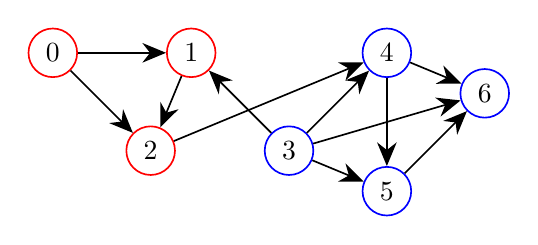
\begin{tikzpicture}[node distance=5em,->,
				-{Stealth[scale=1.5,angle'=45]},semithick]
				\tikzset{state/.style={fill=none, draw=red, text=black,
					shape=circle}}
				\node[state] (0) {0};
				\node[state] (1) [right of=0] {1};
				\node[state] (2) [below right of=0] {2};

				\path 	(0) edge node {} (1)
						(0) edge node {} (2)
						(1) edge node {} (2);
				
				\tikzset{state/.style={fill=none, draw=blue, text=black,
					shape=circle}}
				\node[state] (3) [right of=2] {3};
				\node[state] (4) [above right of=3] {4};
				\node[state] (5) [below of=4] {5};
				\node[state] (6) [above right of=5] {6};

				\path 	(3) edge node {} (4)
						(3) edge node {} (5)
						(3) edge node {} (6)
						(4) edge node {} (5)
						(4) edge node {} (6)
						(5) edge node {} (6);

				\path 	(3) edge node {} (1)
						(2) edge node {} (4);
			\end{tikzpicture}
		\end{center}
		\textbf{Common Local Structures}
		\begin{itemize}
			\item Motifs, repeating local structures, unusually common in 
				biological networks
			\item Some motifs, simplices, are structures in which information 
				flows in one direction, from a `source' node to a `sink' node
		\end{itemize}\footnote{Cite 5,9,11}
		The graph above contains a 2-simplex, in red, and a 3-simplex, in blue.
	\end{posterboxtitle}
	\begin{posterbox}
		\begin{center}\textbf{Graph Convolution}\end{center}
		\begin{itemize}
			\item We designed an algorithm to incorporate information from 
				adjacent nodes in the determination of whether or not a given 
				connection \textit{ij} in a network exists
		\end{itemize}
		\begin{center}
		\begin{tikzpicture}[node distance=5em,->,
			-{Stealth[scale=1.5,angle'=45]},semithick]
			\tikzset{state/.style={fill=none, draw=black, text=black,
				shape=circle}}
				\node[state] (i) {i};
				\node[state] (j) [above right of=1] {j};
				\pgfmathsetmacro\dist{.1em}
				\node (k1) [above=\dist of j] {};
				\node (k2) [above right=\dist of j] {};
				\node (k3) [right=\dist of j] {};
				\node (k4) [below right=\dist of j] {};

				\node (k5) [below=\dist of i] {};
				\node (k6) [above left=\dist of i] {};
				\node (k7) [left=\dist of i] {};
				\node (k8) [below left=\dist of i] {};
				\path 	(j) edge node {} (i)
						(k1) edge node {} (j)
						(k2) edge node {} (j)
						(k3) edge node {} (j)
						(k4) edge node {} (j)
						(i) edge node {} (k5)
						(i) edge node {} (k6)
						(i) edge node {} (k7)
						(i) edge node {} (k8);
		\end{tikzpicture}
		\end{center}

		\vspace{\baselineskip}
	\end{posterbox}
	\begin{posterboxtitle}{Model}
		\noindent\textbf{First Layer}
		\begin{itemize}
			\item Accepts spike-time raster plots for each of \textit{n} neurons
			\item Converts to $(d \times n^2)$ matrix, with each 
				\textit{d}-vector representing one potential edge
			\item Figure here
		\end{itemize}
		\noindent\textbf{Locality Layer}
		\begin{itemize}
			\item Accepts data from the first layer
			\item Incoporates data from potentially adjacent edges into the 
				calculation of the existence of a given edge
			\item Figure here
		\end{itemize}
		\noindent\textbf{Final Layer}
		\begin{itemize}
			\item Converts output from locality layer into $(n \times n)$ 
				adjacency matrix
			\item figure also here
		\end{itemize}
	\end{posterboxtitle}


\end{posterbard}

\end{document}
